\documentclass{beamer}
%\documentclass[trans]{beamer} %om te printen!
%\transglitter etc: kunt ge pas zien op Full Screen (Ctrl+L)

\usepackage{graphicx,multicol}
\usepackage[all]{xy}
\usepackage{graphicx}
\usepackage{beamerouterthememiniframes, beamercolorthemeann,srcltx,hyperref}

\setbeamercolor{normal text}{fg=black!70}
\setbeamertemplate{navigation symbols}{}%geen navigatie
\setbeamertemplate{blocks}[rounded][shadow=true]

%\setbeamercovered{dynamic} %te komen items in lichtgrijs
%\setbeamercolor{background canvas}{bg=black!0}%is wit

\logo{\vspace{-0.2cm}\\
\hfill
\includegraphics[height=3cm]{VUB_schild}}
%plaatst het logo op elke slide onderaan

\newcommand{\Z}{\mathbb{Z}}
\newcommand{\Q}{\mathbb{Q}}
\renewcommand{\P}{\mathbb{P}}
\newcommand{\R}{\mathbb{R}}
\newcommand{\N}{\mathbb{N}}
\newcommand{\C}{\mathbb{C}}
\newcommand{\U}{\mathcal{U}}
\newcommand{\E}{\mathbb{E}}
\newcommand{\z}{\mathcal{Z}}
\newtheorem{remark1}{Remark}
%\columnsep=1.8cm %\columnseprule=.4pt
\newcommand{\cost}{\text{cost}}
\newcommand{\Nash}{\text{Nash}}
\newcommand{\nash}{\text{nash}}
\newcommand{\opt}{\text{opt}}
\newcommand{\copt}{\cost(a_{\opt})}
\title{The Scott Topology}
\author{Filip Moons\\3$^{\text{th}}$ Bachelor of Mathematics\\Promotor: Prof. Dr. Eva Colebunders\\Presentation Bachelor Thesis II}
\date{Friday 19 April, 2013}

\begin{document}

\begin{frame}[plain]

\includegraphics[width=0.4\paperwidth]{VUB_logo.jpg}
\vspace{2cm}
\titlepage
\end{frame}


%\section[Overzicht]{}%rechte haken dienen om niet in de outline te komen
%maar wel vanboven in het donkergroene balkje

%\begin{frame}[plain]{Outline}
%\end{frame}
%
%\begin{frame}[plain]{Outline}
%\tableofcontents[pausesections]
%\end{frame}
%
%
%\section{blabla}
%
%\begin{frame}
%\begin{alertblock}{}
%\begin{center}
%blabla
%\end{center}
%\end{alertblock}
%\end{frame}

\begin{frame}{Content}
\begin{itemize}
  \item Order theory
  \item Load Balancing Games
    \begin{itemize}
    \item Strategic Games: Mixed NE
    \item Congestion Games: Pure NE + Mixed NE
    \item Load Balancing Games: : Pure NE + Mixed NE
    \end{itemize}
  \item Price of Anarchy
  \item Coordination mechanisms
\end{itemize}

\end{frame}


\section{Load Balancing Games}
\subsection{Strategic Games}
\begin{frame}
\begin{definition}
A strategic game $\langle N, (A_i), \succeq_i\rangle$ consists of:
\begin{itemize}
  \item a finite set $N$  (the set of \textbf{players}),
  \item for each player $i \in N$ a nonempty set $A_i$ (the \textbf{set of actions} available to player i),
  \item for each player $i \in N$ a preference relation $\succeq_i$ on $A=\times_{j\in N}A_j$ (the \textbf{preference relation} of player i).
\end{itemize}
\end{definition}
\begin{alertblock}{Remark}
The preference relation  $\succeq_i$ of player $i$ in a strategic game can be represented by a \textbf{payoff function} or \textbf{utility function} $u_i: A \rightarrow \R$, in the sense that $u_i(a) \geq u_i(b)$ whenever $a \succeq_i b$.
\end{alertblock}
\end{frame}
%\begin{frame}
%\begin{block}{}
%\begin{center}
%Introductie
%\end{center}
%\end{block}
%\end{frame}


\begin{frame}{Pure and mixed strategy profiles}
\begin{block}{Pure strategy profile}
$$a = (a_1,...,a_n) \in A, a_i \in A_i$$
\end{block}

\begin{block}{Mixed strategy profile}
$$\alpha = \left(\alpha_i\right)_{i\in N} \in \Delta(A), \alpha_i(a_j) = \P[A_i = a_j]$$
Now,
$$\small{\P[\alpha = a] = \displaystyle\prod_{i \in N} \alpha_i(a_i)}$$
The expected pay off for player $i$ under a mixed strategy profile $\alpha$:
$$\small{U_i(\alpha) = \displaystyle\sum_{a \in A}{\left(\prod_{j \in N}{\alpha_j(a_j)}\right) u_i(a)}}$$
\end{block}

\end{frame}


\begin{frame}{Nash equilibria}
\begin{block}{Pure Nash equilibrum}
A pure strategy profile $a^* \in A$ is a \textbf{pure Nash Equilibrum} if for each player $i\in N$:
$$u_i(a_{-i}^*,a_i^*)) \geq u_i(a_{-i}^*, a_i) \;\;\;\; \forall a_i \in A_i$$
\end{block}

\begin{block}{Mixed Nash equilibrum}
A mixed strategy profile $\alpha^*$ is a \textbf{mixed Nash Equilibrum} if for each player $i \in N$:
$$U_i(\alpha_{-i}^*,\alpha_i^*)) \geq U_i(\alpha_{-i}^*, \alpha_i) \;\;\;\; \forall \alpha_i$$
\end{block}

\end{frame}


\begin{frame}{Theorem of Nash}
\begin{theorem}
Every finite strategic game has a mixed Nash equilibrum.
\end{theorem}
\begin{block}{Lemma: Brouwer fixed point theorem}
Let $X$ be a \emph{\textbf{non-empty}}, convex and compact set. If $f : X \rightarrow X$ is continuous, then there must exist $x \in X$ such that $f(x) = x$.
\end{block}
\begin{block}{Proof.}
$\Delta(A_i)$ is the set of mixed strategy profiles of a player $i$. Note that $(\alpha_i(a_1),..., \alpha_i(a_k))$ with $a_j \in A_i$ (the pure actions of player $i$ are the elements in
$\Delta(A_i)$.
\pause
\begin{itemize}
        \item The set $\Delta(A_i)$ is \textbf{\emph{non-empty}} by definition of a strategic game.
\end{itemize}
\end{block}
\end{frame}


\begin{frame}{Theorem of Nash}
\begin{block}{Lemma: Brouwer fixed point theorem}
Let $X$ be a non-empty, \textbf{\emph{convex}} and compact set. If $f : X \rightarrow X$ is continuous, then there must exist $x \in X$ such that $f(x) = x$.
\end{block}
\begin{block}{Proof.}
\begin{itemize}
         \item To proof that the set $\Delta(A_i)$ is \textbf{\emph{convex}}, take $\vec{x} = (\alpha^x_i(a_1),...,\alpha^x_i(a_k))$ and $\vec{y} = (\alpha^y_i(a_1),...,\alpha^y_i(a_k))$ then $\vec{z} = \theta\vec{x} + (1 - \theta)\vec{y}$ for some $\theta \in [0,1]$ is in $\Delta(A_i)$ because $\vec{z}$ is also a mixed strategy for player $i$ (the sum of the components of $\vec{z}$ is 1).
\end{itemize}
\end{block}
\end{frame}


\begin{frame}{Theorem of Nash}
\begin{block}{Lemma: Brouwer fixed point theorem}
Let $X$ be a non-empty, convex and \textbf{\emph{compact}} set. If $f : X \rightarrow X$ is continuous, then there must exist $x \in X$ such that $f(x) = x$.
\end{block}
\begin{block}{Proof.}
\begin{itemize}
         \item  The \textbf{\emph{compactness}} in $\R^k$ can be shown by proving that the set is closed and bounded. The set is bounded because $0 \leq \alpha_i(a_j) \leq 1$. To proof closeness in $\R^k$, we'll proof that the limit of every convergent sequence in $\Delta(A_i)$ is an element of $\Delta(A_i)$. Consider a convergent sequence in $\Delta(A_i): ((\alpha^n_i(a_1),...,\alpha^n_i(a_k))_n\rightarrow(\alpha^*_i(a_1),...,\alpha^*_i(a_k))$. 

      \end{itemize}
\end{block}
\end{frame}

\begin{frame}{Theorem of Nash}

\begin{block}{Lemma: Brouwer fixed point theorem}
Let $X$ be a non-empty, convex and \emph{\textbf{compact}} set. If $f : X \rightarrow X$ is continuous, then there must exist $x \in X$ such that $f(x) = x$.
\end{block}
\begin{proof}
         $$\sum_{j=1}^k{\alpha^*_i(a_j)}  = \displaystyle\sum_{j=1}^k{\lim_{n\rightarrow\infty}{\alpha^n_i(a_j)}} = \displaystyle\lim_{n\rightarrow\infty}{\sum_{j=1}^k\alpha^n_i(a_j)} = \displaystyle\lim_{n\rightarrow\infty}{1} = 1$$
                        This means that $(\alpha^*_i(a_1),...,\alpha^*_i(a_k))$ is also a mixed strategy for player $i$, but by definition of $\Delta(A_i)$, this limit belongs to $\Delta(A_i)$.
\end{proof}
\end{frame}

\subsection{Congestion Games}
\begin{frame}{Congestion Model}
\begin{definition}
A \textbf{congestion model} $(N, M, (A_i)_{i\in N}, (c_j)_{j\in M})$ is defined as follows:
\begin{itemize}
  \item a finite set $N$ of \textbf{players}. Each player $i$ has a \textbf{weight} (or demand) $w_i \in \N$,
  \item a finite set $M$ of \textbf{facilities}.
  \item For $i \in N$, $A_i$ denotes the set of \textbf{strategies} of player $i$, where each $a_i \in A_i$ is a non-empty \textbf{subset of the facilities},
  \item For $j \in M, c_j$  is a \textbf{cost function} $\N \rightarrow \R$, $c_j(k)$ denotes the cost related to the use of facility $j$ under a certain load $k$;
\end{itemize}
\end{definition}
\end{frame}
\begin{frame}{Congestion Games}
\begin{block}{Definition: Congestion model as strategic game}
\begin{itemize}
 \item a finite set $N$ of \textbf{players},
 \item for each player $i \in N$, there is a nonempty set of  \textbf{strategies} $A_i$,
 \item The preference relation $\succeq_i$ for each player $i$ is defined by a \textbf{payoff function} $u_i: A \rightarrow \R$. For any $a \in A$ and for any $j \in M$, let $\ell_j(a)$ be \emph{the expected load on facility} $j$, assuming $a$ is the current pure strategy profile, so $\ell_j(a) = \sum_{\substack{i \in [n]\\j \in a_i}}{w_i}$ . Then the payoff function for player $i$ becomes: $u_i(a) = \sum_{j\in a_i} c_j(\ell_j(a))$.
  \end{itemize}
\end{block}
\end{frame}
\begin{frame}{Theorem of Rosenthal}
\begin{theorem}
Every congestion game has a pure Nash equilibrium.
\end{theorem}
\end{frame}
\subsection{Load balancing games}
\begin{frame}{Load balancing games}
\begin{definition}
A \textbf{load balancing game} is congestion game based on a congestion model with:
\begin{itemize}
  \item a finite set $N$ of \textbf{tasks} (each task $i$ has a weight $w_i$),
  \item for each player $i \in N$, there is a nonempty set of \textbf{machines}$A_i$ with $A_i \subset M$. The elements of $A_i$ are the possible machines on which task $i$ can be executed.
  \item the preference relation $\succeq_i$ for each client $i$ is defined by a \textbf{payoff function} $u_i: A \rightarrow \R$. For any $a \in A$ and for any $j \in M$, let $\ell_j(a)$ be \emph{the expected load on machine} $j$, assuming $a$ is the current pure strategy profile ($\ell_j(a) = \sum_{\substack{i \in [n]\\j = a_i}}{w_i}$) . Then the payoff function for task $i$ becomes: $u_i(a) = c_{a_i}(\ell_{a_i}(a))$.
\end{itemize}
\end{definition}
\end{frame}
\begin{frame}{Lineair cost functions}
\begin{block}{}
\begin{center}
Payoff function: $u_i(a) = c_{a_i}(\ell_{a_i}(a))$
\end{center}
\end{block}
\begin{block}{}
\begin{center}
Take: $c_{j}(k) = \frac{k}{s_j}$, $s_j$: speed of machine $j$.
\end{center}
\end{block}

\begin{block}{Pure strategies}
The \textbf{\emph{payoff function}}:
$$u_i(a) = c_{a_i}(\ell_{a_i}(a)) =  \frac{\ell_{a_i}(a)}{s_{a_i}}, a \in A$$
The \emph{\textbf{makespan}}: $$\cost(a)=\max_{j\in[m]}{c_j(\ell_j(a))} = \max_{j\in[m]}{\frac{\ell_{j}(a)}{s_{j}}}$$
\end{block}

\end{frame}



\begin{frame}{Lineair cost functions}
\begin{block}{}
\begin{center}
Payoff function: $u_i(a) = c_{a_i}(\ell_{a_i}(a))$
\end{center}
\end{block}
\begin{block}{}
\begin{center}
Take: $c_{j}(k) = \frac{k}{s_j}$, $s_j$: speed of machine $j$.
\end{center}
\end{block}

\begin{block}{Mixed strategies}
The \textbf{\emph{expected payoff function}}:
$$U^j_i(\alpha) = \frac{w_i + \sum_{k\neq i}{w_k\alpha_k(j)}}{s_j} $$
The \emph{\textbf{makespan}}:
$$\cost(\alpha) = \E[\cost(a)] = \E\left[\max_{j\in[m]}\frac{\ell_j(a)}{s_{j}}\right]$$
\end{block}
\end{frame}

\begin{frame}{A very easy example}
\begin{columns}[t]
\column{5.3cm}
\begin{alertblock}{Figure}
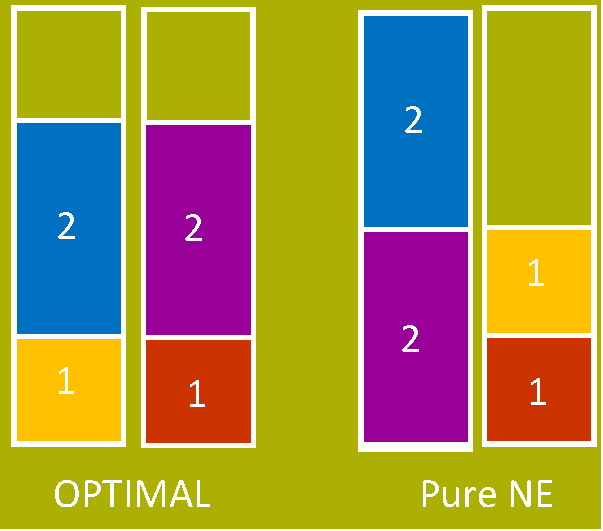
\includegraphics[scale=0.5]{figuurpresentatie.pdf}
\end{alertblock}

\column{5.5cm}
\begin{itemize}
\item $\copt = \max(3,3) = 3$
\item $\cost(a_2) = \max(4,4) = 4$
\end{itemize}
\end{columns}
\end{frame}

\section{Price of Anarchy}
\subsection{Concept}
\begin{frame}{Definition}
\begin{definition}
$$PoA(G) = \displaystyle\max_{\alpha \in \Nash(G)} {\frac{\cost(\alpha)}{\cost(a_{\opt})}}$$
\end{definition}
\end{frame}


\begin{frame}{A very easy example}
\begin{columns}[t]
\column{5.3cm}
\begin{alertblock}{Figure}
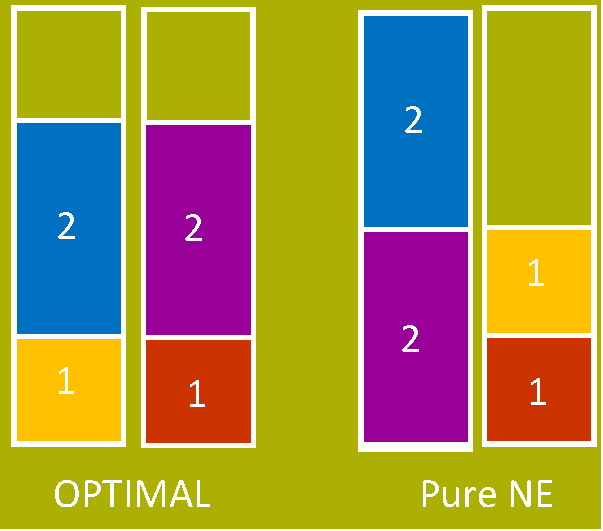
\includegraphics[scale=0.5]{figuurpresentatie.pdf}
\end{alertblock}

\column{5.5cm}
\begin{itemize}
\item $PoA(G)= \frac{4}{3} = 1.33$
\end{itemize}
\end{columns}
\end{frame}

\subsection{Bounds on $PoA$}
\begin{frame}{Bachmann-Landau notations}
\begin{block}{Definition: Big Oh}
Big Oh is the set of all functions $f$ that are bounded above by $g$ asymptotically (up to constant factor).
$$O(g(n)) = \{f|\exists c, n_0 \geq 0: \forall n \geq n_0 : 0 \leq f(n) \leq cg(n)\}$$
\end{block}
\begin{block}{Definition: Asymptotical equality}
Let $f$ and $g$ real functions, then $f$ is asymptotically equal to $g$ $\Leftrightarrow \displaystyle\lim_{x\rightarrow +\infty} \frac{f(x)}{g(x)}=1$. Notation: $f \sim g$.
\end{block}
\end{frame}

\begin{frame}{$PoA$ in Pure Nash equilibria on uniformly related machines}

\begin{lemma}
$\forall m \in \R: \Gamma^{-1}(m) \in O\left(\frac{\log m}{\log \log m}\right)$.
\end{lemma}
\begin{block}{Proof.}
$\Gamma(z) = \int_0^\infty  t^{z-1} e^{-t}\,{\rm d}t$, $\Gamma^{-1}(m) = k$, then $k!$ is the greatest factorial smaller or equal to $m$. Because $m \sim k!$ and $k! \sim k^k$ we get:
\vspace{-.8cm}
\begin{eqnarray*}
&\Rightarrow& m \sim k^{k} \\
&\Rightarrow& \log m \sim k\log(k) \\
&\Rightarrow& k \sim \frac{\log m}{\log(k)}\\
&\Rightarrow& k \sim \frac{\log m}{\log(\frac{\log m}{\log (k)})}
\end{eqnarray*}

\end{block}


\end{frame}

\begin{frame}{$PoA$ in Pure Nash equilibria on uniformly related machines}

\begin{lemma}
$\forall m \in \R: \Gamma^{-1}(m) \in O\left(\frac{\log m}{\log \log m}\right)$.
\end{lemma}
\begin{block}{Proof.}
$\Gamma(z) = \int_0^\infty  t^{z-1} e^{-t}\,{\rm d}t$, $\Gamma^{-1}(m) = k$, then $k!$ is the greatest factorial smaller or equal to $m$. Because $m \sim k!$ and $k! \sim k^k$ we get:
\vspace{-.8cm}
\begin{eqnarray*}
&\Rightarrow& m \sim k^{k} \\
&\Rightarrow& \log m \sim k\log(k) \\
&\Rightarrow& k \sim \frac{\log m}{\log(k)}\\
&\Rightarrow& k \sim \frac{\log m}{\log(\frac{\log m}{\log (k)})}
\end{eqnarray*}

\end{block}


\end{frame}
\begin{frame}{$PoA$ in Pure Nash equilibria on uniformly related machines}

\begin{lemma}
$\forall m \in \R: \Gamma^{-1}(m) \in O\left(\frac{\log m}{\log \log m}\right)$.
\end{lemma}

\begin{proof}
\vspace{-.4cm}
\begin{eqnarray*}
&\Rightarrow& k \sim \frac{\log m}{\log\log m - \log\log (k)}
\end{eqnarray*}
Because $m > k$:
$$\Rightarrow k \sim \frac{\log m}{\log \log m}$$

So that $\Gamma^{-1}(m) \in O\left(\frac{\log m}{\log \log m}\right)$
\end{proof}
\end{frame}

\begin{frame}{Summary}

\begin{center}
\begin{tabular}{l|c|c}

  % after \\: \hline or \cline{col1-col2} \cline{col3-col4} ...
   & Identical & Uniformly related \\
   \hline

   \hline
  Pure NE & $2-\frac{2}{m+1}$ & $\Theta\left(\frac{\log m}{\log \log m}\right)$ \\
  \hline
  Mixed NE & $\Theta\left(\frac{\log m}{\log \log m}\right)$ & $\Theta\left(\frac{\log m}{\log \log \log m}\right)$ \\
  \hline
\end{tabular}
\end{center}

\end{frame}

\section{Coordination Mechanisms}
\subsection{Policies}
\begin{frame}{Policies}
\begin{itemize}
 \item \textbf{Shortest first}
  \item \textbf{Longest first}
  \item \textbf{Random order}
  \item \textbf{Round Robin}
 \end{itemize}
  \begin{theorem} Under a longest-first policy, PoA for uniformly related machines is $\leq 2 - \frac{2}{m+1}$.
\end{theorem}

\begin{theorem} Under a shortest-first policy, PoA for uniformly related machines is $\Theta(\log m)$
\end{theorem}
\end{frame}
\subsection{Taxation}
\begin{frame}{Taxation}
\begin{block}{Definition: Tax function}
$\delta: M \times \R \rightarrow \R$
\end{block}
\end{frame}
\section*{Bibliography}
\begin{frame}
\begin{itemize}
 \item B. V\"{o}cking, \emph{Selfish Load Balancing}, Chapter 20 in Algorithmic Game Theory, Cambridge University Press, December 2007.
\item d J. Osborne and A. Rubinstein, \emph{A course in Game Theory},  The MIT Press, 1994.
\item S. Mannor, \emph{Advancded Topics in Systems, Learning and Control, Lecture 3: Lecture 3: Mixed Actions, Nash and Correlated Equilibria}, Technicon, November 2008.
\item E. Colebunders, \emph{Analyse II}, Vrije Universiteit Brussel, 2011.
\item C. Witteveen, Intreerede: De Prijs van de Onafhankelijkheid, TU Delft 2007.
\item Y. Mansour, \emph{Lecture 6: Congestion and potential games}, Computational Learning Theory, University of Tel Aviv, 2003.
\item Jason R. Marden, \emph{Lecture 12: Game Theory Course}, University of Colorado.
\item T. Harks, M. Klimm, R. H. M\"{o}hring, \emph{Characterizing the Existence of Potential Functions in Weighted Congestion Games}, February 2011
\end{itemize}
\end{frame}

\begin{frame}
\begin{itemize}
\item R. W. Rosenthal, \emph{ A class of games possessing pure-strategy Nash equilibria}. International Journal of Game Theory, 2:65–67, 1973
\item K. Etessami, \emph{Algorithmic Game Theory - Lecture 16 Best response dynamics and pure Nash Equilibria}, University of Edingburgh, 2007.

\item I. Caragiannis, C. Kaklamanis, P. Kanellopoulos, \emph{Improving the Efficiency of Load Balancing Games through Taxes}, University of Patras, 2008.

\item S. Suri, C. D. T\'{o}th, Y. Zhou. \emph{Selfish Load Balancing and Atomic Congestion Games}, University of California, 2004.
\item W. De Meuter. \emph{Algoritmen en Datastructuren I}, Vrije Universiteit Brussel, 2011.
\item K.G. Binmore. \emph{Mathematical Analysis: A Straightforward Approach}, Cambridge Universitiy Press, 1977.
\item Galambos, J\'{a}nos, Simonelli. \emph{Bonferroni-Type Inequalities with Applications, Probability and Its Applications}, Springer-Verlag, 1996.
\end{itemize}
\end{frame}

\end{document}
